\section{ME1/1 Chambers}
\label{app:me11}

The innermost ME1/1 station should provide very good spatial resolution of 75 $\mu$m per
station in order to achieve the required momentum resolution in the endcap muon system. The
chambers must provide efficient pattern recognition and matching with the inner tracker. This
spatial resolution should be delivered in the presence of a strong axial magnetic field in excess
of 3 Tesla. The chambers should be very fast in order to identify the bunch-crossing. Their
recovery time should be fast because the chambers will operate in the presence of the highest
particle background rate in the CMS Muon System, up to 1 kHz/cm$^2$, which corresponds to a
rate of 100 kHz per cathode readout channel.

The design parameters of the ME1/1 CSCs are optimized to meet the specified
requirements. A general view of the chamber is shown in Fig. \ref{fig:me11_overview}

To compensate for the Lorentz effect of the axial magnetic field at a
nominal value of 3.8 Tesla, the anode wires are positioned at an inclination angle of 29$^o$ with
respect to and perpendicular to the central strip axis

\begin{figure}[htb]
  \begin{center}
    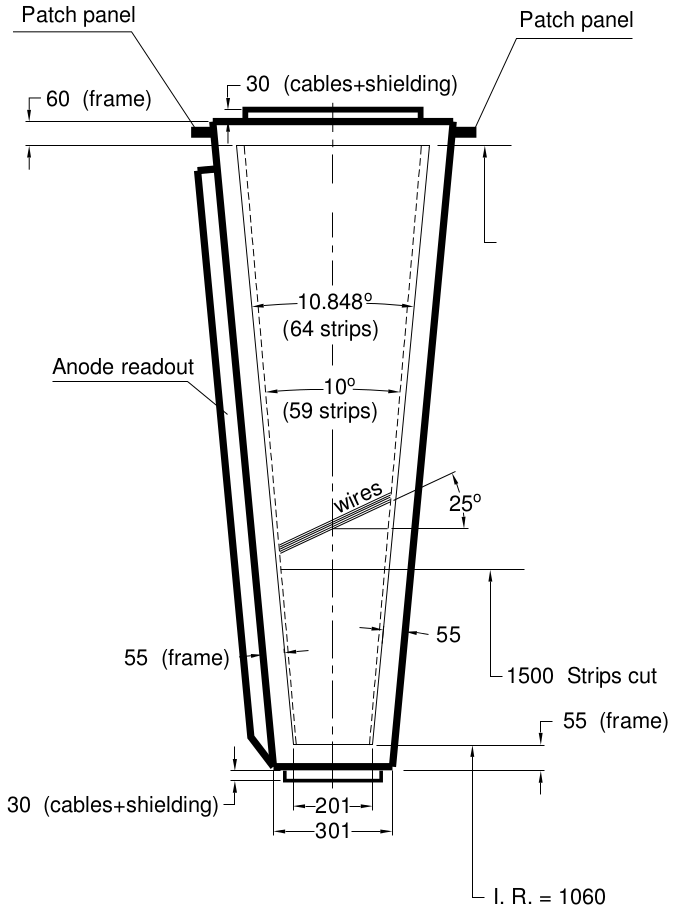
\includegraphics[width=0.70\linewidth]{figures/ME11_overview.png}
    \caption{ME11 chamber specifications}
    \label{fig:me11_overview}
  \end{center}
\end{figure}